\documentclass[12pt]{article}

\usepackage[spanish]{babel}
\usepackage[utf8]{inputenc}
\usepackage{graphicx}
\usepackage{geometry}
\usepackage{xcolor}
\usepackage{fancyhdr}
\usepackage{lastpage}
\usepackage{pdfpages}
\usepackage{listings}

\geometry{top=25mm,left=15mm,right=15mm,a4paper}

\pagestyle{fancy}
\fancyhf{}
\lhead{Seminario de Ciencias de la Computación A}
\cfoot{Página \thepage\ de \pageref{LastPage}}

\graphicspath{./}

\begin{document}
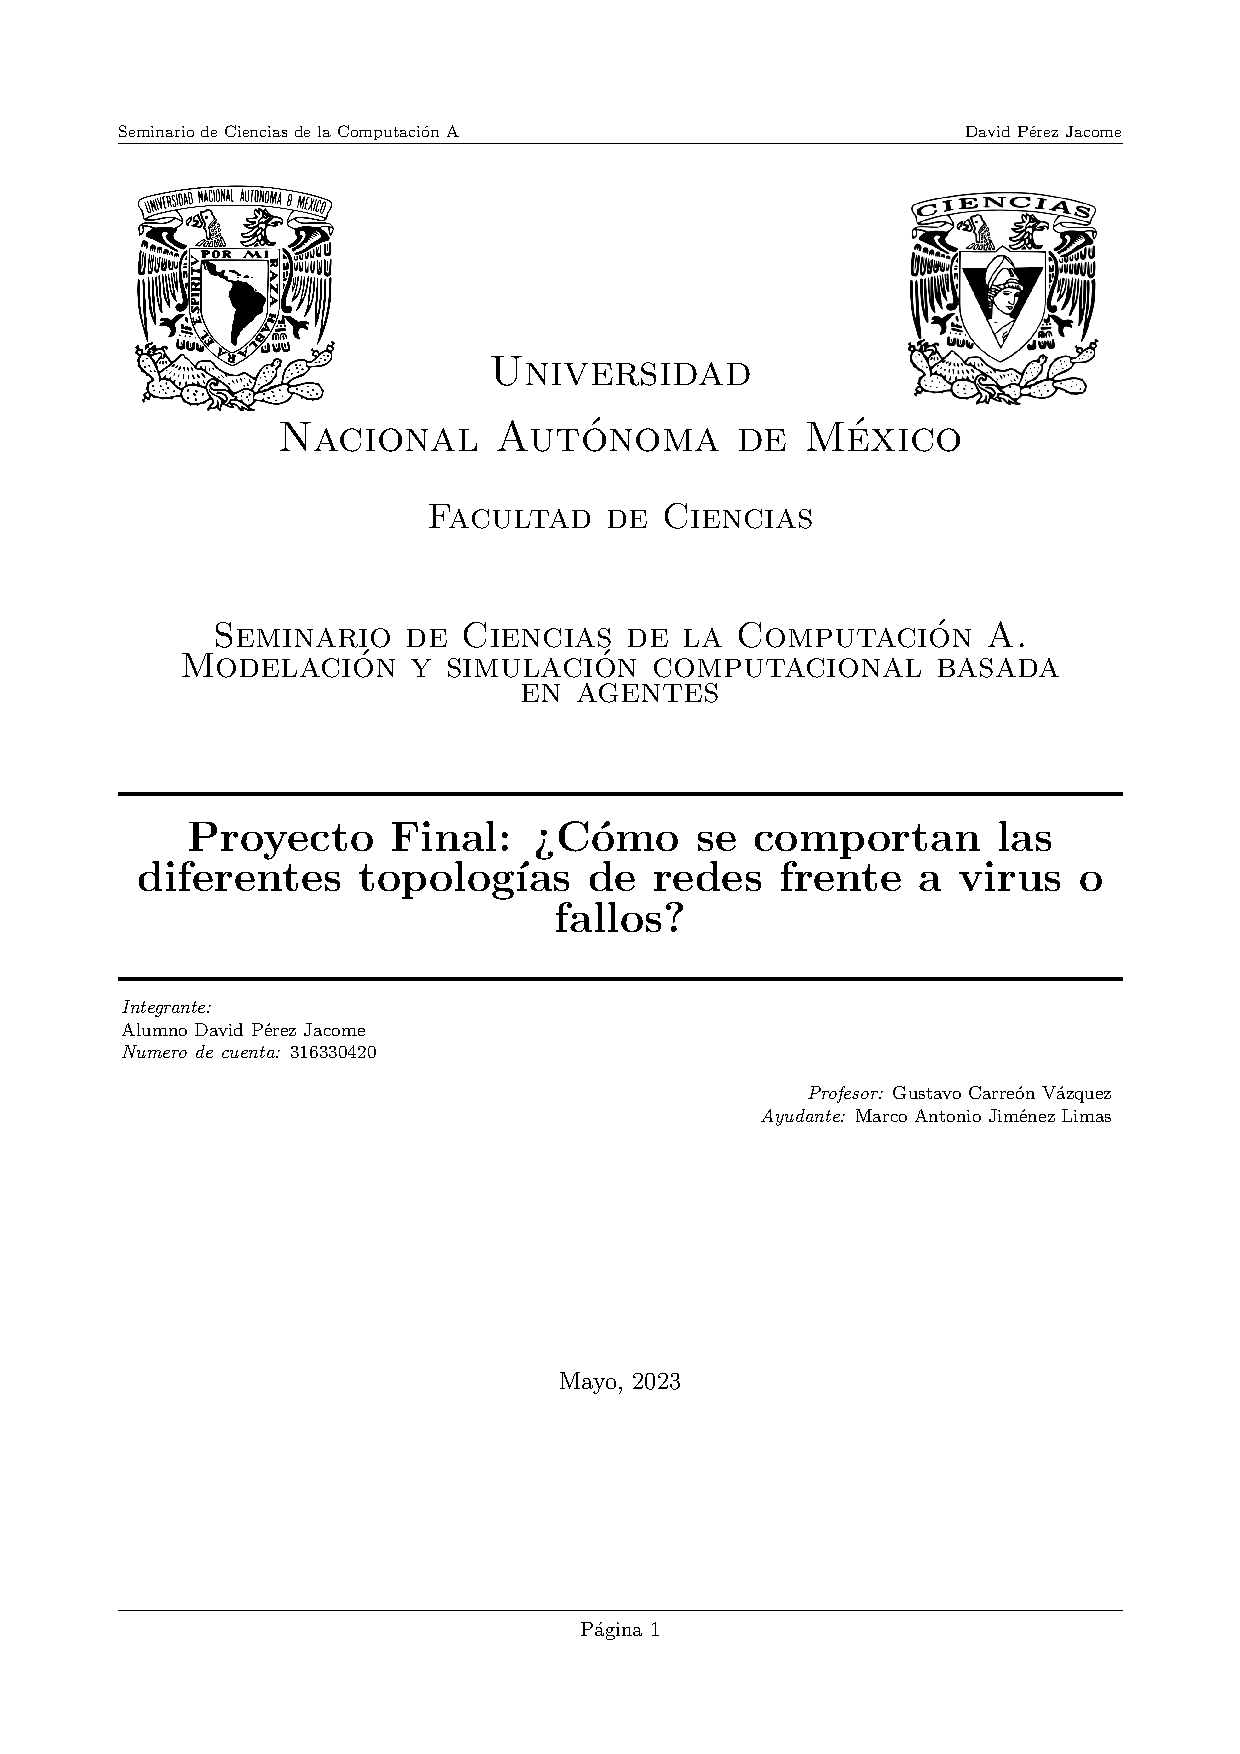
\includepdf{Portada.pdf}
{\color{red} \section*{Proyecto Final: ¿Cómo se comportan las diferentes topologías de redes frente a virus o fallos?.}}
\vspace{2em}

{\color{blue} \subsection*{1- INTRODUCCIÓN.}}
\vspace{1em}

¿Cómo se comportan las diferentes topologías de redes frente a virus o fallos?, esta es la pregunta a la que a lo largo de este trabajo nos vamos a dedicar a responder.
A lo largo del curso de Modelación Basada en Agentes hemos ido aprendiendo diversas aplicaciones y simulaciones del mundo real en las que podemos "modelar" y mostrar el como es el comportamiento de algún fenomeno
ya sea fisico o en este caso computacional, en este trabajo abordaremos principalmente la problematica de modelar una estructura de red, pero para ello debemos tener presente que es un sistema de redes, que en pocas palabras una red de ordenadores se refiere a dispositivos de computación 
interconectados que pueden intercambiar datos y compartir recursos entre sí. 
Los dispositivos de la red utilizan un sistema de reglas, llamados protocolos de comunicaciones, para transmitir información a través de tecnologías físicas o inalámbricas.\\

También veremos el comportamiento dado fallos en diferentes topologias de red, pero para esto debemos de tener presente que es la topología de redes, la topología de redes es la disposición de nodos y enlaces se denomina topología de red. Se pueden configurar de diferentes maneras para obtener diferentes resultados. Algunos tipos de topologías de red son:\\
\begin{enumerate}
    \item Bus: Cada nodo solo está vinculado a otro nodo. La transmisión de datos a través de las conexiones de red se produce en una dirección.
    \item Anillo: Cada nodo está vinculado a otros dos nodos, formando un anillo. Los datos pueden fluir de manera bidireccional. Sin embargo, el error de un solo nodo puede provocar la caída de toda la red.
    \item Estrella: Un nodo de servidor central está vinculado a múltiples dispositivos de red de clientes. Esta topología funciona mejor ya que los datos no tienen que pasar por cada nodo. También es más fiable.
    \item Malla: Cada nodo está conectado a muchos otros nodos. En una topología de malla completa, cada nodo está conectado a todos los demás nodos de la red.
\end{enumerate}

En las redes computacionales existen asi como diversos tipos de topologías, distintos tipos de fallos o infecciones via virus, para este proyecto nos enfocaremos principalmente en como se ve afectada la red dado un contagio que puede ser relacionado a un virus o a un fallo en el sistema, en general y para hacer un poco mas sencillo de entender y de implmenetar el sistema, vamos a utilizar un fallo similar a una infección via algún virus.
Pero es importante decir que no es lo mismo; Podemos definir los fallos o eventos de una red como aquellos sucesos que interfieren en el correcto funcionamiento de la red, y por consiguiente disminuyen significativamente su rendimiento. Los ejemplos de fallos más comunes incluyen fallos en el hardware, en el cableado, interferencia inalámbrica, así como un cambio en el estado del puerto, saturación de ancho de banda o, lo que es peor, la pérdida de conectividad.
Mientras que un virus informático es una aplicación o código malintencionado que se emplea para ejecutar actividades destructivas en un dispositivo o red local. La actividad malintencionada de este código puede dañar el sistema local de archivos, robar datos, interrumpir servicios, descargar más malware o cualquier otra acción que esté codificada en el programa. Muchos virus simulan ser programas legítimos para convencer a los usuarios de que los ejecuten en su dispositivo, insertando así la carga útil del virus.
En el que podemos de manera similiar utilizar el modelo SIR para su modelación.\\

Para este modelo nos apoyaremos de la biblioteca de modelos de NetLogo, el modelo \textbf{Virus on a Network} para no complicar tanto el modelo, de igualmanera por el tiempo y poder tener una base solida de la implementación.\\
Es importante modelar este tipo de comportamiento especifico en las redes ya que en ocaciones al tener una red de computadoras tan compleja como lo son la mayoria si no es que todas, y nos resulta que un componente de nuestro sistema tiene una falla, 
el como se debe de abordar tal problematica es de suma importancia para que el sistema siga con su proceso de comunicación apesar de la o las fallas que resulten, para que nuestro sistema no llegue a caer.\\

El modelar este tipo de comportamientos nos ayudan para saber el timpo de mantenimiento que le debemos de dar al sistema en si para que no ocacione fallas catastroficas que compromentan todo el sistema, asi mismo podemos ver en el modelo como es que se comunican los componentes del sistema a pesar de una falla o contagio.\\

En otros modelos que he visto este tipo de fallos los han abordado con distintos algoritmos distribuidos, estos algoritmos son también "Detectores de fallos", de igual manera es posible implmentar usando Modelación Basada en Agentes, este tipo de comportamiento de envio-recepción de mensajes. que trataremos de abordar de manera "implicita" en nuestro sistema.\\

En modelos basados en agentes este tipo de problemas de redes los han abordado de manera diferente, usando como lo mencione anteriomente diferentes tipos de algoritmos distribuidos, para esto explicaremos que es un algoritmo distribuido. 













{\color{blue} \subsection*{2- PLANTEAMIENTO.}}
\vspace{1em}


{\color{blue} \subsection*{3- DESARROLLO.}}
\vspace{1em}

{\color{blue} \subsection*{4- RESULTADOS.}}
\vspace{1em}

{\color{blue} \subsection*{5- CONCLUSIONES Y REFLEXIONES.}}
\vspace{1em}

{\color{blue} \subsection*{6- BIBLIOGRAFIA.}}
\vspace{1em}

\begin{thebibliography}{99}
    \bibitem{1}
    Amazon Web Services. (s.f.). What is Computer Networking? Recuperado de https://aws.amazon.com/es/what-is/computer-networking/
    \bibitem{2}
    SciELO México. (2015). Los modelos basados en agentes y su aplicación en el estudio de los sistemas socio-ambientales. Scientia Et Technica, 20(3), 227-232. Recuperado de $https://www.scielo.org.mx/scielo.php?script=sci_arttext\&pid=S0185-19182015000300227$
    \bibitem{3}
    CIC. (s.f.). ¿Qué es Network Fault Management o la Gestión de Fallos de Red? Recuperado de https://www.cic.es/que-es-network-fault-management-o-la-gestion-de-fallos-de-red/

\end{thebibliography}



\end{document}